\documentclass{beamer}
\usetheme{Warsaw}
\usepackage{tikz}
\usepackage{minted}
\usefonttheme{professionalfonts}
\usecolortheme{sidebartab}
\usetikzlibrary{chains, shadows.blur, trees}
%Information to be included in the title page:
\title[\url{https://llvm.org/}] %optional
{LLVM \& Clang}

\subtitle{LLVM : Low Level Virtual Machine}

\author[LLVM \& Clang] % (optional, for multiple authors)
{Presented By Sumit~Lahiri\inst{1} \& Nitesh Trivedi\inst{1}}

\institute[VFU] % (optional)
{
	\inst{1}%
	IIT Kanpur
}

\date[] % (optional)
{Hands On Session for \texttt{LLVM} \& \texttt{clang}}

\begin{document}
\frame{\titlepage}

\begin{frame}
	\frametitle{LLVM}
	\begin{itemize}
		\item LLVM : Low Level Virtual Machine. \pause
		\item Compiler Infrastructure. \pause
		\item Frontend : \texttt{clang}, C++, C, go, java to AST and finally to LLVM-IR. \pause
		\item Middle End : \texttt{opt tool}, Optimizations and other passes on LLVM-IR. \pause
		\item Back End : \texttt{LLVM CodeGen/Backend}, LLVM-IR to target code generator.  \pause
	\end{itemize}
\end{frame}

\begin{frame}[fragile]
	\frametitle{Clang AST}
	\begin{minted}[fontsize=\footnotesize, tabsize=2,linenos]{cpp}
int retsum(int a, int b) {
	return a + b;
}
# clang -Xclang -ast-dump -fsyntax-only code.cpp
`-FunctionDecl <test.cc:1:1, line:3:1> retsum 'int (int, int)'
	|-ParmVarDecl <col:12, col:16> col:16 used a 'int'
	|-ParmVarDecl <col:19, col:23> col:23 used b 'int'
		`-CompoundStmt <col:26, line:3:1>
			`-ReturnStmt <line:2:3, col:14>
				`-BinaryOperator <col:10, col:14> 'int' '+'
					|-ImplicitCastExpr <col:10> 'int' <LValueToRValue>
						| `-DeclRefExpr <col:10> 'int' lvalue ParmVar 'a' 'int'
					`-ImplicitCastExpr <col:14> 'int' <LValueToRValue>
						`-DeclRefExpr <col:14> 'int' lvalue ParmVar 'b' 'int'
	\end{minted}
\end{frame}

\begin{frame}[fragile]
	\frametitle{Clang AST}
	\begin{minted}[fontsize=\footnotesize, tabsize=2,linenos]{cpp}
int main() 
{ 
	int a = 90;
}
# ./clang_ast "int main() { int a = 90; }"
FunctionDecl 0x3705db0 <input.cc:1:1, col:26> col:5 main 'int ()'
	`-CompoundStmt 0x3705f78 <col:12, col:26>
		`-DeclStmt 0x3705f60 <col:14, col:24>
			`-VarDecl 0x3705ed8 <col:14, col:22> col:18 a 'int' cinit
				`-IntegerLiteral 0x3705f40 <col:22> 'int' 90
	\end{minted}
\end{frame}

\begin{frame}[fragile]
	\frametitle{AST Visual}
\begin{minted}[fontsize=\footnotesize, tabsize=2]{cpp}
	x > 0xff2 
	
	|-BinaryOperator 0x3c32fb0 '_Bool' '>'
	| |-ImplicitCastExpr 0x3c32f98 'int' <LValueToRValue>
	| | `-DeclRefExpr 0x3c32f58 'int' lvalue Var 0x3c32ed8 'x' 'int'
	| `-IntegerLiteral 0x3c32f78 'int' 4082
	
\end{minted}
	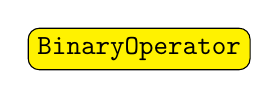
\begin{tikzpicture}[auto,level distance=1cm,
		level 1/.style={sibling distance=4cm},
		level 2/.style={sibling distance=3.5cm},
		level 3/.style={sibling distance=3.2cm},
		level 4/.style={sibling distance=1.9cm},
		level 5/.style={sibling distance=1cm},
		level 6/.style={sibling distance=0.5cm},
		box/.style = {draw,rounded corners,align=center}]
		\node [box, fill=yellow, text=black]{\texttt{BinaryOperator}};
	\end{tikzpicture}
\end{frame}

\begin{frame}[fragile]
	\frametitle{AST Visual}
\begin{minted}[fontsize=\footnotesize, tabsize=2]{cpp}
	x > 0xff2 
	
	|-BinaryOperator 0x3c32fb0 '_Bool' '>'
	| |-ImplicitCastExpr 0x3c32f98 'int' <LValueToRValue>
	| | `-DeclRefExpr 0x3c32f58 'int' lvalue Var 0x3c32ed8 'x' 'int'
	| `-IntegerLiteral 0x3c32f78 'int' 4082
	
\end{minted}
			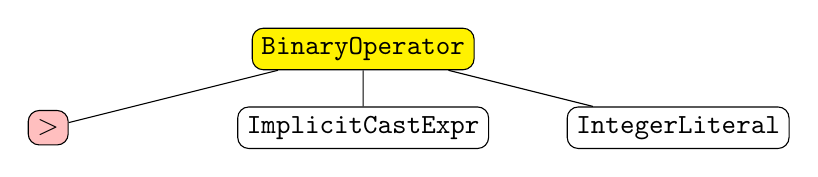
\begin{tikzpicture}[auto,level distance=1cm,
			level 1/.style={sibling distance=4cm},
			level 2/.style={sibling distance=3.5cm},
			level 3/.style={sibling distance=3.2cm},
			level 4/.style={sibling distance=1.9cm},
			level 5/.style={sibling distance=1cm},
			level 6/.style={sibling distance=0.5cm},
			box/.style = {draw,rounded corners,align=center}]
			\node [box, fill=yellow, text=black]{\texttt{BinaryOperator}}
			child {node [box, fill=pink, text=black] {$>$}}
			child {node [box, fill=white, text=black] {\texttt{ImplicitCastExpr}}
			}
			child {node [box, fill=white, text=black] {\texttt{IntegerLiteral}}
			};
		\end{tikzpicture}
\end{frame}

\begin{frame}[fragile]
	\frametitle{AST Visual}
\begin{minted}[fontsize=\footnotesize, tabsize=2]{cpp}
	x > 0xff2 
	
	|-BinaryOperator 0x3c32fb0 '_Bool' '>'
	| |-ImplicitCastExpr 0x3c32f98 'int' <LValueToRValue>
	| | `-DeclRefExpr 0x3c32f58 'int' lvalue Var 0x3c32ed8 'x' 'int'
	| `-IntegerLiteral 0x3c32f78 'int' 4082
	
\end{minted}
	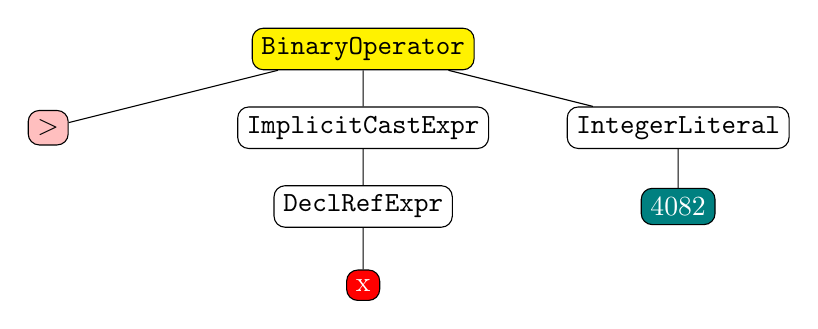
\begin{tikzpicture}[auto,level distance=1cm,
		level 1/.style={sibling distance=4cm},
		level 2/.style={sibling distance=3.5cm},
		level 3/.style={sibling distance=3.2cm},
		level 4/.style={sibling distance=1.9cm},
		level 5/.style={sibling distance=1cm},
		level 6/.style={sibling distance=0.5cm},
		box/.style = {draw,rounded corners,align=center}]
		\node [box, fill=yellow, text=black]{\texttt{BinaryOperator}}
		child {node [box, fill=pink, text=black] {$>$}}
		child {node [box, fill=white, text=black] {\texttt{ImplicitCastExpr}}
			child {node [box, fill=white, text=black] {\texttt{DeclRefExpr}} 
				child {node [box, fill=red, text=white] {x}}
			}
		}
		child {node [box, fill=white, text=black] {\texttt{IntegerLiteral}}
			child {node [box, fill=teal, text=white] {4082}}
		};
	\end{tikzpicture}
\end{frame}

\begin{frame}[fragile]
	\frametitle{LLVM IR}
	\begin{minted}[fontsize=\footnotesize, tabsize=2,linenos]{cpp}
int retsum(int a, int b) {
	return a + b;
}
# clang -S -emit-llvm code.cpp -O0 -o code.ll
; ModuleID = 'test.cc'
source_filename = "test.cc"
target datalayout = "e-m:e-p270:32:32-p271:32:32-p272:64:64-i64:..."
target triple = "x86_64-unknown-linux-gnu"

; Function Attrs: mustprogress noinline nounwind optnone uwtable
define dso_local i32 @_Z6retsumii(i32 %0, i32 %1) #0 {
	%3 = alloca i32, align 4
	%4 = alloca i32, align 4
	store i32 %0, i32* %3, align 4
	store i32 %1, i32* %4, align 4
	%5 = load i32, i32* %3, align 4
	%6 = load i32, i32* %4, align 4
	%7 = add nsw i32 %5, %6
	ret i32 %7
}
	\end{minted}
\end{frame}

\begin{frame}
	\frametitle{LLVM Pass}
	\begin{itemize}
		\item Primarily analyze and transform the LLVM intermediate representation. \pause
		\item Eg : Run your own optimization on the LLVM IR. \pause
		\item Get the IR representation using \texttt{-S -emit-llvm} flags. \pause
		\item Transformation Pass -- Modify the CFG. Extract Useful info. \texttt{-licm, -dce}\pause
		\item Analysis Pass -- Run analysis on the BBs of CFG. \texttt{-domtree, -dot-cfg}\pause 
		\item Utility Pass -- View/Log some information from CFG. \pause
		\item Run on \texttt{Module} \pause or \texttt{Function}. \pause
		\begin{itemize}
			\item Code up pass logic in \texttt{struct} inherited from \texttt{PassInfoMixin}, \pause must have a \texttt{run()} function. \pause
			\item Register the \texttt{Pass} and build your pass into a shared library which can be loaded and used by \texttt{opt} tool to run pass on LLVM IR. 
		\end{itemize}
	\end{itemize}
\end{frame}

\begin{frame}[fragile]
	\frametitle{LLVM Pass}
	\begin{minted}[fontsize=\footnotesize, tabsize=2,linenos]{cpp}
struct MyPass : public PassInfoMixin<MyPass> {
	PreservedAnalyses run(Function \&F, FunctionAnalysisManager \&FM){
		# Your code logic	
		...
		return PreservedAnalyses::all();
	}
	...
};
extern "C" ::llvm::PassPluginLibraryInfo LLVM_ATTRIBUTE_WEAK
llvmGetPassPluginInfo() {
	return {LLVM_PLUGIN_API_VERSION, "MyPass", "v0.1",
		[](PassBuilder &PB) {
			PB.registerPipelineParsingCallback(
			[](StringRef Name, FunctionPassManager &FPM,
			ArrayRef<PassBuilder::PipelineElement>) {
				if (Name == "mypass") {
					FPM.addPass(ModifyBuildCFG());
					return true;
				}
				return false; }); }};
}
	\end{minted}
\end{frame}

\begin{frame}[fragile]
	\frametitle{LLVM Pass}
	\begin{minted}[fontsize=\footnotesize, tabsize=2,linenos]{cpp}
struct MyPass : public PassInfoMixin<MyPass> {
	PreservedAnalyses run(Module \&T, ModuleAnalysisManager \&M){
		# Your code logic	
		...
		return PreservedAnalyses::all();
	}
	...
};
extern "C" ::llvm::PassPluginLibraryInfo LLVM_ATTRIBUTE_WEAK
llvmGetPassPluginInfo() {
	return {LLVM_PLUGIN_API_VERSION, "MyPass", "v0.1",
		[](PassBuilder &PB) {
			PB.registerPipelineParsingCallback(
			[](StringRef Name, ModulePassManager &MPM,
			ArrayRef<PassBuilder::PipelineElement>) {
				if (Name == "mypass") {
					MPM.addPass(ModifyBuildCFG());
					return true;
				}
				return false; }); }};
}
	\end{minted}
\end{frame}

\begin{frame}
	\frametitle{Clang Frontend Pass AKA ClangAST Frontend Action}
	\begin{itemize}
		\item Input is the source code, i.e. \texttt{C/C++/go} file. \pause
		\item Abstract Syntax Tree which can be traversed. \pause
		\item Run a \texttt{FrontEnd} action on the AST. \pause
		\item Representation : \texttt{Stmt}, \pause \texttt{Decl} \pause or \texttt{Expr}. \pause
		\item Start from the \texttt{TopLevelDecl} or \texttt{TranslationUnitDecl} \pause and recursively parse down. \pause
		\item Clang Plugin or Standalone tool (\texttt{clang LibTooling}).
	\end{itemize}
\end{frame}

\begin{frame}
	\frametitle{Clang Frontend Pass AKA ClangAST Frontend Action}
		\begin{itemize}
			\item \texttt{ASTFrontendAction} : Interface to define Action to be performed on the AST. \pause
			\item \texttt{ASTConsumer} : Consumes the AST, ASTFrontendAction creates a consumer. \pause
			\item Handles what function to run or what to do with each \texttt{TranslationUnit}. \pause
			\item \texttt{RecursiveASTVisitor} : Consumer can use a visitor to visit each \texttt{Decl} Node and perform certain actions. \pause
			\item Finally we build our logic into a tool using \texttt{CommonOptionsParser} \& \texttt{ClangTool}. \pause
		\end{itemize}
\end{frame}

\begin{frame}[fragile]
	\frametitle{Clang ASTFrontendAction}
		\begin{minted}[fontsize=\footnotesize, tabsize=2,linenos]{cpp}
class ClassAction : public clang::ASTFrontendAction {
	public:
	# returns a uniq ptr to your consumer.
	virtual std::unique_ptr<clang::ASTConsumer>
	CreateASTConsumer(clang::CompilerInstance &Compiler, 
		llvm::StringRef InFile) {
		return 
			# Instantiate your consumer. 
			std::make_unique<ClassConsumer>(
				&Compiler.getASTContext()
			);
	}
};
	\end{minted}
\end{frame}

\begin{frame}[fragile]
	\frametitle{Clang ClassConsumer}
	\begin{minted}[fontsize=\footnotesize, tabsize=2,linenos]{cpp}
class ClassConsumer : public clang::ASTConsumer {
	public:
		explicit ClassConsumer(ASTContext *Context) 
			: Visitor(Context) {}
		virtual void HandleTranslationUnit(clang::ASTContext &Context) {
			# Called on each TranslationDeclUnit
			Visitor.TraverseDecl(Context.getTranslationUnitDecl());
		}
	private:
		# Implements the actual recursive visit strategy.
		ClassVisitor Visitor;
};
	\end{minted}
\end{frame}

\begin{frame}[fragile]
	\frametitle{Clang ClassConsumer}
	\begin{minted}[fontsize=\footnotesize, tabsize=2,linenos]{cpp}
class ClassVisitor
: public RecursiveASTVisitor<ClassVisitor> {
public:
	explicit FindNamedClassVisitor(ASTContext *Context) 
		: Context(Context) {}
	
	bool VisitWhileStmt(WhileStmt *S) {
		llvm::outs() << "While Condition : ";
		if (S)
		VisitDecl(S->getConditionVariable());
		return true;
	}
	# ... More Visit Logic. 
	bool VisitDecl(clang::Decl *Declaration) {
		Declaration->dump();
		return true;
	}

private:
	ASTContext *Context;
};
	\end{minted}
\end{frame}

\end{document}